\documentclass[tikz,convert={outext=.svg,command=\unexpanded{pdf2svg \infile\space\outfile}},multi=false]{standalone}
\usepackage[utf8]{inputenc}

\usetikzlibrary{automata}% tikz package already loaded by 'tikz' option
\begin{document}


\newcommand\xm5
\newcommand\xM{10}
\newcommand{\ensembleequations}{
$\begin{array}{ll}
1\cdot x & = x \\
x^{-1}\cdot x & = 1 \\
(x\cdot y) \cdot z & = x \cdot (y \cdot z)
\end{array}$}

\newcommand{\monsystemedereecriture}{
$\begin{array}{ll}
1\cdot x &  \rightarrow x \\
x^{-1}\cdot x &  \rightarrow 1 \\
(x\cdot y) \cdot z&  \rightarrow x \cdot (y \cdot z) \\
x^{-1} \cdot (x \cdot y) & \rightarrow y \\
1^{-1} & \rightarrow 1 \\
x \cdot 1&  \rightarrow x \\
(x^{-1})^{-1} & \rightarrow x \\
x \cdot x^{-1} & \rightarrow 1 \\
x \cdot (x^{-1} \cdot y) & \rightarrow y \\
(x \cdot y)^{-1}&  \rightarrow y^{-1} x^{-1}
\end{array}$~~~~}

\newcommand\ok{%
\raisebox{-1mm}{%

\begin{tikzpicture}[scale=0.5]
\node [circle, fill=green!70!black, minimum height=5mm] at (0.3, -0.1) {};
\draw[line width=0.8mm, white] (0, 0) -- (0.2, -0.3) -- (0.6, 0.1);
\end{tikzpicture}}}
\newcommand\notok{%
\raisebox{-1mm}{%

\begin{tikzpicture}
\node [circle, fill=red!80!black, minimum height=5mm] at (0.1, 0.09) {};
\draw[line width=0.8mm, white] (0, 0) -- (0.2, 0.2);
\draw[line width=0.8mm, white] (0.2, 0) -- (0, 0.2);
\end{tikzpicture}}}


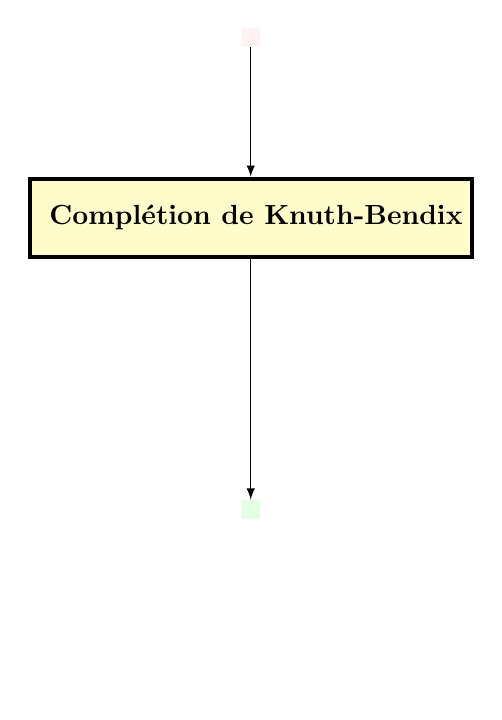
\begin{tikzpicture}
%\node (m) at (0, -1) {Un ensemble d'équations};
\node[fill=red!5] (m)  at (0, -1) { \ensembleequations};


\node[minimum height=1cm, draw, line width=0.5mm, fill=yellow!20] (mc) at (0, -3.3) {\textbf{~Complétion de Knuth-Bendix~}};
\draw[-latex] (m) -- (mc);
%\node [] (r) at (0, -5) {Un système de réécriture confluent et terminant};
\node [fill=green!10] (r) at (0, -7) {\monsystemedereecriture};
\node []  at (2.4, -9.2) {\ok};
\draw[-latex] (mc) -- (r);

\end{tikzpicture}
\end{document}